\begin{subsectionframemod}{Difference between Natural and Aerial Images}
    \metroset{block=fill}
    \begin{alertblock}{SVF (Singular Value Fine-tuning)}
        SVF (Singular Value Fine-tuning) est une technique d'ajustement des modèles de réseaux neuronaux qui réduit la complexité en décomposant les matrices de poids en valeurs singulières.
        En ne modifiant que les valeurs singulières les plus importantes, elle permet d'améliorer l'efficacité tout en limitant l'overfitting, en évitant d'ajuster un trop grand nombre de paramètres.
    \end{alertblock}

    \begin{figure}
        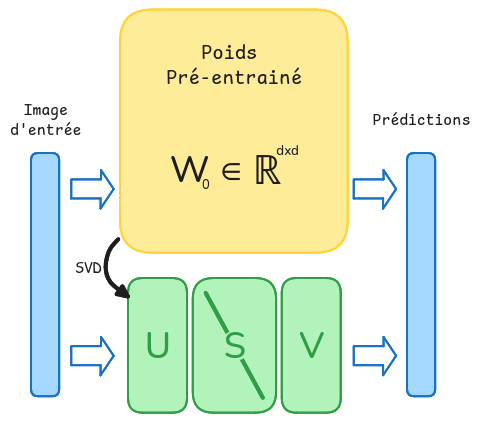
\includegraphics[width=0.4\textwidth]{Figures/svf.png}
        \caption{Principe de l'entrainement SVF. Ici on entraine seulement les valeurs propres (\cite{sun2022singular}).}
    \end{figure}


\end{subsectionframemod}